\documentclass[lanscape, 10pt,twoside,a4paper]{article}
% http://www-h.eng.cam.ac.uk/help/tpl/textprocessing/latex_maths+pix/node6.html symboles de math
% http://fr.wikibooks.org/wiki/Programmation_LaTeX Programmation latex (wikibook)
%=========================== En-Tete =================================
%--- Insertion de paquetages (optionnel) ---
\usepackage[french]{babel}   % pour dire que le texte est en fran{\'e}ais
\usepackage{a4}	             % pour la taille   
\usepackage[T1]{fontenc}     % pour les font postscript
\usepackage{epsfig}          % pour gerer les images
%\usepackage{psfig}
\usepackage{amsmath, amsthm} % tres bon mode mathematique
\usepackage{amsfonts,amssymb}% permet la definition des ensembles
\usepackage{float}           % pour le placement des figure
\usepackage{verbatim}

\usepackage{multicol} % multicolonnes

\usepackage{longtable} % pour les tableaux de plusieurs pages

\usepackage[table]{xcolor} % couleur de fond des cellules de tableaux

\usepackage{lastpage}

\usepackage{multirow}

\usepackage{multicol} % pour {\'e}crire dans certaines zones en colonnes : \begin{multicols}{nb colonnes}...\end{multicols} 

% \usepackage[top=1.5cm, bottom=1.5cm, left=1.5cm, right=1.5cm]{geometry}
% gauche, haut, droite, bas, entete, ente2txt, pied, txt2pied
\usepackage{vmargin}
\setmarginsrb{0.20cm}{0.20cm}{0.20cm}{0.20cm}{15pt}{3pt}{42pt}{15pt}

	
\usepackage{pdflscape}
\usepackage{lscape} % changement orientation page
%\usepackage{frbib} % enlever pour obtenir references en anglais
% --- style de page (pour les en-tete) ---
\pagestyle{empty}

% mettre du texte en diagonale sur le fond : tikz
\usepackage{tikz} 
\def\confidentialTIKZ{%
	\begin{tikzpicture}[remember picture,overlay]
	\node[rotate=60,scale=15,text opacity=0.1] at (current page.center) {Confidentiel};
	\end{tikzpicture}
}%

\def\TIKZcyberpunkRED{%
	\begin{tikzpicture}[remember picture,overlay]
	\node[rotate=60,scale=10,text opacity=0.1] at (current page.center) {Cyberpunk RED};
	\end{tikzpicture}
}%

\def\txtTITLE{Feuille de personnage Cyberpunk RED} %%%%% !! TITRE !! %%%%%
\def\imgCORNER{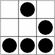
\includegraphics[width=0.25cm]{../../../../images/glider/logo-glider.png}}

\def\imgGLIDERLEFTT{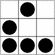
\includegraphics[width=1.95cm]{../../../../images/glider/logo-glider-left.png}}
\def\imgGLIDERRIGHT{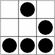
\includegraphics[width=1.95cm]{../../../../images/glider/logo-glider-right.png}}

\def\imgGLIDERLEFTTsmall{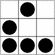
\includegraphics[width=0.25cm]{../../../../images/glider/logo-glider-left.png}}
\def\imgGLIDERRIGHTsmall{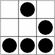
\includegraphics[width=0.25cm]{../../../../images/glider/logo-glider-right.png}}

% % % en-tete et pieds de page configurables : fancyhdr.sty

% http://www.trustonme.net/didactels/250.html

% http://ww3.ac-poitiers.fr/math/tex/pratique/entete/entete.htm
% http://www.ctan.org/tex-archive/macros/latex/contrib/fancyhdr/fancyhdr.pdf
\usepackage{fancyhdr}
\pagestyle{fancy}
	% \renewcommand{\chaptermark}[1]{\markboth{#1}{}}
	% \renewcommand{\sectionmark}[1]{\markright{\thesection\ #1}}
\fancyhf{}
\fancyhead[LE,RO]{\bfseries\thepage \TIKZcyberpunkRED }
\fancyhead[LO]{\bfseries\rightmark}
\fancyhead[RE]{\bfseries\leftmark}
\fancyfoot[LE]{\thepage /\pageref{LastPage} \hfill
	\scriptsize{\txtTITLE} % TITLE
\hfill \imgGLIDERLEFTTsmall }
\fancyfoot[RO]{\imgGLIDERRIGHTsmall \hfill
	\scriptsize{\txtTITLE} % TITLE
\hfill \thepage /\pageref{LastPage}}
\renewcommand{\headrulewidth}{0.5pt}
\renewcommand{\footrulewidth}{0.5pt}
\addtolength{\headheight}{0.5pt}
% \fancypagestyle{plain}{
	% \fancyhead{}
	% \renewcommand{\headrulewidth}{0pt}
% }

\def\smallbox{%
	\setlength{\unitlength}{0.5cm}
	\fbox{
		\begin{picture}(1, 1)(0,0)
		\end{picture}
	}
}%

%%%%%%%%%%% SOME VALUES IN ENGLISH %%%%%%%%%%%%%%%%%%%%%
\def\ENdefNom{\textbf{Name} \dotfill }


%%%%%%%%%%% QUELQUES VALEURS EN FRANCAIS %%%%%%%%%%%%%%%%%%%%%
\def\FRdefNom{\small \textbf{Nom} \dotfill }
\def\FRdefRole{\small \textbf{R{\^o}le} \dotfill }
\def\FRdefPPerso{\small \textbf{Points de \newline Personnage} \dotfill }
\def\FRdefCaract{\small \textbf{Caract{\'e}ristiques} \dotfill }
\def\FRdefLocali{\small \textbf{Localisation \newline Armure PA} \dotfill }
\def\FRdefSauveg{\small \textbf{Sauvegarde} \hrulefill \dotfill }
\def\FRdefMCMCMC{\small \textbf{MC} \hrulefill \dotfill }
\def\FRdefBonusD{\small \textbf{Bonus Domages} \hrulefill \dotfill }
\def\FRdefCOMPET{\small \textbf{Comp{\'e}tences} \dotfill }

%%%%% exchange (find & replace) between 'ENdef' end 'FRdef' from here to forward (43 occurences) %%%%%

\def\CELblackTXTWhite{\cellcolor{black} \color{white}}


%============================= Corps =================================
\begin{document}
\begin{landscape}

\setlength\parindent{0pt}

%% \small

\begin{tabular}{ p{0.20\textwidth} p{0.07\textwidth} p{0.32\textwidth} p{0.32\textwidth} p{0.32\textwidth} } 
	\begin{tabular}{ p{0.20\textwidth} }
		\footnotesize
		%% CyberPunk RED --- Fiche de personnage \\
		\fbox{ \begin{minipage}[ht]{0.20\textwidth} 
			-- 
			\newline \newline \newline \newline \newline 
			\newline \newline \newline \newline \newline
			\newline \newline \newline \newline \newline
		\end{minipage} } \\ 
		\fbox{ \begin{minipage}[ht]{0.20\textwidth} 
			Pseudo \newline
		\end{minipage} } \\ 
		\fbox{ \begin{minipage}[ht]{0.20\textwidth} 
			Rôle \newline
		\end{minipage} } \\ 
		\fbox{ \begin{minipage}[ht]{0.20\textwidth} 
			Capacité de Rôle	---	Rang \newline
		\end{minipage} } \\
		\fbox{ \begin{minipage}[ht]{0.20\textwidth}
			NOTES
			\newline \newline \newline \newline \newline
		\end{minipage} } \\ 
		\fbox{ \begin{minipage}[ht]{0.20\textwidth} 
			Humanité	--- SUR --- \newline
		\end{minipage} } \\
	\end{tabular}
	& ~ 
	\begin{tabular}{ p{0.07\textwidth} }
		\footnotesize
		\fbox{ \begin{minipage}[ht]{0.07\textwidth} 
			INT \newline \newline 
		\end{minipage} } \\
		\fbox{ \begin{minipage}[ht]{0.07\textwidth} 
			RÉF \newline \newline 
		\end{minipage} } \\ 
		\fbox{ \begin{minipage}[ht]{0.07\textwidth} 
			DEX \newline \newline 
		\end{minipage} } \\ 
		\fbox{ \begin{minipage}[ht]{0.07\textwidth} 
			TECH \newline \newline 
		\end{minipage} } \\ 
		\fbox{ \begin{minipage}[ht]{0.07\textwidth} 
			PRES \newline \newline 
		\end{minipage} } \\ 
		\fbox{ \begin{minipage}[ht]{0.07\textwidth} 
			VOL \newline \newline 
		\end{minipage} } \\ 
		\fbox{ \begin{minipage}[ht]{0.07\textwidth} 
			CHA \newline \newline 
		\end{minipage} } \\ 
		\fbox{ \begin{minipage}[ht]{0.07\textwidth} 
			MOUV \newline \newline 
		\end{minipage} } \\ 
		\fbox{ \begin{minipage}[ht]{0.07\textwidth} 
			COR \newline \newline 
		\end{minipage} } \\ 
		\fbox{ \begin{minipage}[ht]{0.07\textwidth} 
			EMP \newline \newline 
		\end{minipage} } \\ 
	\end{tabular}
	& ~ 
	\begin{tabular}{ p{0.32\textwidth} }
		%% Table Compétence 1/3
		\fbox{ \begin{minipage}[ht]{0.32\textwidth}
			\footnotesize
			\begin{tabular}{|p{0.48\textwidth}|c|c|c|}
				\hline
				\CELblackTXTWhite 
				Compétences de Contrôle					&	NIV		&	CAR		&	BAS		\\
				\hline
				Conduite de véhicule Terrestre (RÉF)	&			&			&		 	\\
				\hline
				Équitation (RÉF)						&			&			&		 	\\
				\hline
				Pilotage de véhicule aérien (x2) (RÉF)	&			&			&		 	\\
				\hline
				Pilotage de véhicule maritime (RÉF)		&			&			&		 	\\
				\hline
			\end{tabular}

			\begin{tabular}{|p{0.48\textwidth}|c|c|c|}
				\hline
				\CELblackTXTWhite 
				Compétences \newline de Combat			&	NIV		&	CAR		&	BAS		\\
				\hline
				Arme de mêlée (DEX)						&			&			&		 	\\
				\hline
				Art martial (x2) (DEX)					&			&			&		 	\\
				\hline
				Bagarre (DEX)							&			&			&		 	\\
				\hline
				Esquive (DEX)							&			&			&		 	\\
				\hline
			\end{tabular}
			
			\begin{tabular}{|p{0.48\textwidth}|c|c|c|}
				\hline
				\CELblackTXTWhite 
				Compétences de Corps					&	NIV		&	CAR		&	BAS		\\
				\hline
				Athlétisme (DEX)						&			&			&		 	\\
				\hline
				Contorsion (DEX)						&			&			&		 	\\
				\hline
				Danse (DEX)								&			&			&		 	\\
				\hline
				Discrétion (DEX)						&			&			&		 	\\
				\hline
				Endurance (VOL)							&			&			&		 	\\
				\hline
				Résistance torture / drogues (VOL)		&			&			&		 	\\
				\hline
			\end{tabular}
			
			\begin{tabular}{|p{0.48\textwidth}|c|c|c|}
				\hline
				\CELblackTXTWhite 
				Compétences \newline d'Éducation		&	NIV		&	CAR		&	BAS		\\
				\hline
				Bibliothèque (INT)						&			&			&		 	\\
				\hline
				Bureaucratie (INT)						&			&			&		 	\\
				\hline
				Composition (INT)						&			&			&		 	\\
				\hline
				Comptabilité (INT)						&			&			&		 	\\
				\hline
				Connaissance (INT)						&			&			&		 	\\
				\hline
				Criminoologie (INT)						&			&			&		 	\\
				\hline
				Cryptographie (INT)						&			&			&		 	\\
				\hline
				Déduction (INT)							&			&			&		 	\\
				\hline
				Dressage (INT)							&			&			&		 	\\
				\hline
				Gestion d’affaires (INT)				&			&			&		 	\\
				\hline
				Jeux de hasard (INT)					&			&			&		 	\\
				\hline
			\end{tabular}
			%% --- 
		\end{minipage} } \\ 
	\end{tabular}
	& ~ 
	\begin{tabular}{ p{0.32\textwidth} }
		%% Table Compétence 2/3
		\fbox{ \begin{minipage}[ht]{0.32\textwidth}
			\footnotesize
			\begin{tabular}{|p{0.48\textwidth}|c|c|c|}
				\hline
				\CELblackTXTWhite 
				Compétences \newline d'Éducation		&	NIV		&	CAR		&	BAS		\\
				\hline
				Guide Local (INT)						&			&			&		 	\\
				\hline
				$\Rightarrow$ Quartier d'origine		&			&			&		 	\\
				\hline
				$\Rightarrow$ 							&			&			&		 	\\
				\hline
				$\Rightarrow$ 							&			&			&		 	\\				
				\hline
				Langue (INT)							&			&			&		 	\\
				\hline
				$\Rightarrow$ Argot						&			&			&		 	\\
				\hline
				$\Rightarrow$ 							&			&			&		 	\\
				\hline
				$\Rightarrow$ 							&			&			&		 	\\	
				\hline
				Science (INT)							&			&			&		 	\\
				\hline
				$\Rightarrow$ 							&			&			&		 	\\
				\hline
				$\Rightarrow$ 							&			&			&		 	\\	
				\hline
				Survie en milieu hostile (INT)			&			&			&		 	\\
				\hline
				Tactique (INT)							&			&			&		 	\\
				\hline				
			\end{tabular}
			
			\begin{tabular}{|p{0.48\textwidth}|c|c|c|}
				\hline
				\CELblackTXTWhite 
				Compétences \newline de représentration	&	NIV		&	CAR		&	BAS		\\
				\hline
				Instrument (TECH)						&			&			&		 	\\
				\hline
				$\Rightarrow$ 							&			&			&		 	\\
				\hline
				$\Rightarrow$ 							&			&			&		 	\\				
				\hline
				$\Rightarrow$ 							&			&			&		 	\\				
				\hline
				$\Rightarrow$ 							&			&			&		 	\\				
				\hline
				Jeu d'acteur (PRES)						&			&			&		 	\\
				\hline				
			\end{tabular}
			
			\begin{tabular}{|p{0.48\textwidth}|c|c|c|}
				\hline
				\CELblackTXTWhite 
				Compétences \newline de Sociabilité		&	NIV		&	CAR		&	BAS		\\
				\hline
				Connaissance de la rue (PRES)			&			&			&		 	\\
				\hline
				Conversation (EMP)						&			&			&		 	\\
				\hline
				Corruption (PRES)						&			&			&		 	\\
				\hline
				Habillement et Style (PRES)				&			&			&		 	\\
				\hline
				Interrogatoire (PRES)					&			&			&		 	\\
				\hline
				Look (PRES)								&			&			&		 	\\
				\hline
				Négoce (PRES)							&			&			&		 	\\
				\hline
				Persuasion (PRES)						&			&			&		 	\\
				\hline
				Psychologie (EMP)						&			&			&		 	\\
				\hline
			\end{tabular}
			%% --- 
		\end{minipage} } \\ 
	\end{tabular}
	& ~ 
	\begin{tabular}{ p{0.32\textwidth} }
		Table Compétence 2/3
		\fbox{ \begin{minipage}[ht]{0.32\textwidth}
			\footnotesize
			\begin{tabular}{|p{0.48\textwidth}|c|c|c|}
				\hline
				\CELblackTXTWhite 
				Compétences \newline de Technique		&	NIV		&	CAR		&	BAS		\\
				\hline
				Aérotech (TECH)							&			&			&		 	\\
				\hline
				Aérotech (TECH)							&			&			&		 	\\
				\hline
				Aérotech (TECH)							&			&			&		 	\\
				\hline
				Aérotech (TECH)							&			&			&		 	\\
				\hline
			\end{tabular}
			--- 
		\end{minipage} } \\ 
	\end{tabular}
	\\
	
	%% TODO Deux colonnes : Points de santé, blessures...
	
	%% TODO trois colonnes : Armes et armures
	
	%% TODO page 2 (parcours) (équipement)
	
	%% TODO page 3 CYBERMATÉRIEL
\end{tabular}


\end{landscape}

\end{document}
